\documentclass[usenames,dvipsnames, 18pt, compress, aspectratio=169]{beamer}

% can be compiled by xelatex -shell-escape presentation.tex
% lualatex -shell-escape presentation.tex

\usepackage[utf8]{inputenc}
\usepackage[english]{babel}
\usepackage{booktabs}
\usepackage[scale=2]{ccicons}
\usepackage{listings}
\usepackage{marvosym}
\usepackage{color}
\usepackage{xcolor}
\usepackage[document]{ragged2e}
\usepackage[export]{adjustbox}
\usepackage{fontawesome5}
\usepackage{enumitem}
\usepackage{minted}
\usemintedstyle{tango}
\usepackage[normalem]{ulem}
\usepackage{tikz}
\usetikzlibrary{
    shapes,
    positioning,
    fit
}

\usepackage[nott]{inconsolata}
\usepackage{graphicx}
\usepackage{eso-pic}
\usepackage{verbatim}
\usepackage{smartdiagram}
\usesmartdiagramlibrary{additions}
\usepackage{datetime}
\usepackage{hyperref}
\usepackage{forloop}
\usepackage{csquotes}

\usepackage{tcolorbox}
\usepackage{tabularx}
\usepackage{array}
\usepackage{colortbl}
\tcbuselibrary{skins}

\usetikzlibrary{shapes,arrows,positioning}
\graphicspath{{images}}

\def\twitter{{\faTwitter}}
\def\github{{\faGithub}}
\def\email{{\faEnvelope}}

\renewcommand{\ttdefault}{pcr}
%\newfontfamily{\ttfamily}{SourceCodePro-Regular}

\usefonttheme{professionalfonts} % using non standard fonts for beamer
\usefonttheme{serif} % default family is serif
\usepackage{fontspec}
\setmainfont{Liberation Sans}
\newfontfamily\ExtraLight{Liberation Sans}
\newfontfamily\Light{Liberation Sans}
\newfontfamily\Book{Liberation Sans}
\newfontfamily\Medium{Liberation Sans}
\setmonofont{FiraCode-VF}

\makeatletter
\newcommand\HUGE{\@setfontsize\Huge{32}{41}}
\makeatother

\newcommand\AtPagemyUpperLeft[1]{\AtPageLowerLeft{%
\put(\LenToUnit{0.85\paperwidth},\LenToUnit{0.05\paperheight}){#1}}}

\newcommand\AtPagemyUpperTop[1]{\AtPageLowerLeft{%
\put(\LenToUnit{0.42\paperwidth},\LenToUnit{0.90\paperheight}){#1}}}

\renewcommand{\ULthickness}{2.0pt}

\definecolor{links}{HTML}{0099FF}
\hypersetup{colorlinks, linkcolor=, urlcolor=links}
\definecolor{title}{HTML}{ee0000}

\setbeamerfont{section title}{family=\Book, size=\Huge, shape=\normalfont}
\setbeamerfont{frametitle}{family=\Book, size=\large, shape=\normalfont}
\setbeamerfont{title}{family=\Book, size=\Large, shape=\normalfont}
\setbeamerfont{subtitle}{size=\small}
\setbeamerfont{author}{family=\ExtraLight, size=\footnotesize}

\setbeamercolor{frametitle}{fg=black}
\setbeamertemplate{frametitle}[default][center]
\setbeamerfont{frametitle}{size=\Large, series=\bfseries}

\setbeamersize{text margin left=0mm,text margin right=0mm}

\setbeamertemplate{navigation symbols}{}
\beamertemplatenavigationsymbolsempty
\pagenumbering{gobble}

\setbeamertemplate{title page}
{

  \vspace*{2.1cm}
  \hspace{7.0cm}
  \begin{minipage}[b][\paperheight]{0.5\textwidth}
  \begin{center}

    \ifx\inserttitle\@empty\else
    {{% \inserttitle is nonempty
      \raggedright%
      %\linespread{1.0}%
      \usebeamerfont{title}%
      \usebeamercolor[fg]{title}%
      %\vspace*{1.3em}
      \if@noSmallCapitals%
        \inserttitle%
      \else%
        \scshape{\color{title} \textbf{\begin{flushleft}\inserttitle\end{flushleft}}}%
      \fi%
      \vspace*{0.3em}
    }}
    \fi

    \vspace*{0.5em}%

    \ifx\insertsubtitle\@empty\else
    {{% \insertsubtitle is nonempty
      \usebeamerfont{subtitle}%
      \usebeamercolor[fg]{subtitle}%
      {\color{black} \insertsubtitle}%
      \vspace*{3.0em}%
    }}
    \fi

    \vspace*{1.0em}%

    \usebeamerfont{author}%
    \usebeamercolor[fg]{author}%
    {\begin{flushleft}\color{black} \insertauthor\end{flushleft}}%

    %\vspace*{1.5em}
    \fontsize{8pt}{10}\selectfont
    {\begin{flushleft}\color{black} 12-09-2022\end{flushleft}}%

    \vfill
    \vspace*{2em}
  \end{center}
  \end{minipage}
}

\setbeamertemplate{section page}
{
  \vspace{2em}
  \centering
  \begin{minipage}{22em}
    \usebeamercolor[fg]{section title}
    \usebeamerfont{section title}
    {\color{black} \insertsectionhead\\[-1ex]}
  \end{minipage}
  \par
}

\setbeamertemplate{footline}
{
\begin{beamercolorbox}[wd=\textwidth,ht=3ex,dp=3ex,leftskip=0.3cm,rightskip=0.3cm]{structure}
  \usebeamerfont{page number in head/foot}
  \insertframenumber
\end{beamercolorbox}
}

\title{Performance Insights into eBPF Step by Step}
\subtitle{}
\date{\today}
\author{Dmitrii Dolgov\\ Senior Software Engineer}
\institute{}

\tikzset{page/.style={
    draw,
    fill=gray!30,
    rounded corners=.1cm,
}}

\tikzset{prog/.style={
    draw,
    fill=yellow!30,
    minimum height=1.0cm,
    minimum width=1.8cm,
    %rounded corners=.25cm,
}}

\tikzset{app/.style={
    draw,
    fill=blue!30,
    minimum height=2cm,
    minimum width=2cm,
    rounded corners=.55cm,
}}

\tikzset{kernel/.style={
    draw,
    fill=green!30,
    minimum height=2cm,
    minimum width=2cm,
    rounded corners=.55cm,
}}

\tikzset{bpf/.style={
    draw,
    fill=red!30,
    minimum height=2cm,
    minimum width=2cm,
    rounded corners=.55cm,
}}

\tikzset{connection/.style={
    draw=none
}}

\tikzset{arrow/.style={
    ->,>=stealth,
    line width=0.2mm,
    color=red!50,
}}

\begin{document}
{
  \usebackgroundtemplate{
\includegraphics[width=\paperwidth]{title.png}}%
  \fontsize{17pt}{18}\selectfont
  \maketitle
}

\AddToShipoutPictureBG{
  \AtPagemyUpperLeft{{
\includegraphics[width=2.0cm,keepaspectratio]{logo.png}}}
}

\setbeamertemplate{background canvas}{}

\fontsize{17pt}{18}\selectfont

\begin{frame}[fragile]{}
    \frametitle{}

    \begin{center}
        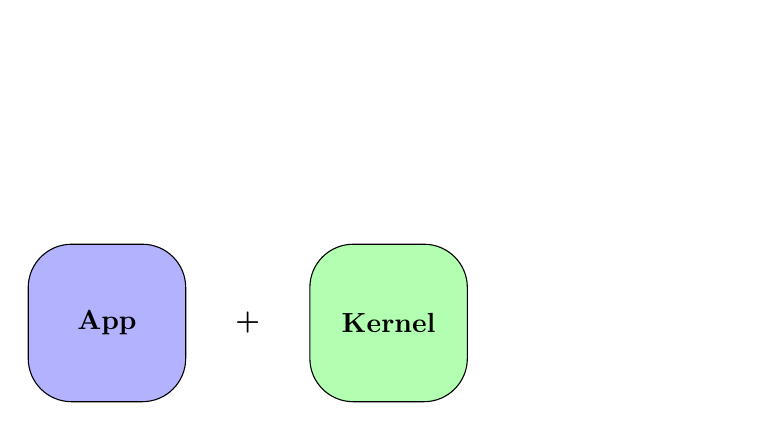
\begin{tikzpicture}[
                align=center,
                node distance=0.0cm
        ]
            \node[app] (app) {\textbf{App}};
            \node[connection, right=0.5cm of app] (plus1) {\textbf{+}};

            \node[kernel, right=0.5cm of plus1] (kernel) {\textbf{Kernel}};
            \node[connection, right=0.5cm of kernel, color=white, draw opacity=0, line width=0] (plus2) {\textbf{+}};

            \node[bpf, right=0.5cm of plus2, color=white, draw opacity=0] (bpf) {\textbf{BPF ?}};
            \node[connection, draw=none, color=white, draw opacity=0, line width=0, above=1cm of kernel] (hot-path) {Hot Path};
            \draw[arrow, draw opacity=0, line width=0, color=white, draw=none] (hot-path) to [out=60,in=90] (bpf);

        \end{tikzpicture}
    \end{center}
\end{frame}

\begin{frame}[fragile]{}
    \frametitle{}

    \begin{center}
        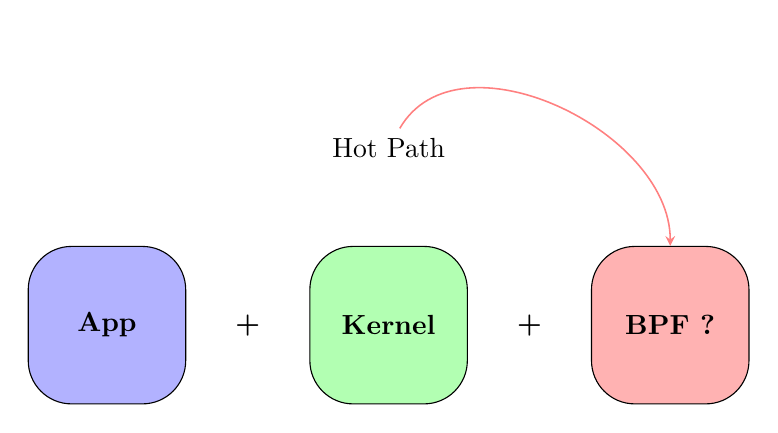
\begin{tikzpicture}[
                align=center,
                node distance=0.0cm
        ]
            \node[app] (app) {\textbf{App}};
            \node[connection, right=0.5cm of app] (plus1) {\textbf{+}};

            \node[kernel, right=0.5cm of plus1] (kernel) {\textbf{Kernel}};
            \node[connection, right=0.5cm of kernel] (plus2) {\textbf{+}};

            \node[bpf, right=0.5cm of plus2] (bpf) {\textbf{BPF ?}};
            \node[connection, above=1cm of kernel] (hot-path) {Hot Path};
            \draw[arrow] (hot-path) to [out=60,in=90] (bpf);

        \end{tikzpicture}
    \end{center}
\end{frame}

\fontsize{26pt}{26}\selectfont
\begin{frame}[fragile]{}
    \frametitle{}

    \begin{center}
        Current state of things
    \end{center}
\end{frame}

\fontsize{17pt}{18}\selectfont

\begin{frame}[fragile]{}
    \frametitle{BPF Instruction Set}

    \begin{center}
        \begin{minted}[fontsize=\large]{c}
                       if (delta < ts)
        \end{minted}

        \vspace{0.5cm}

        \begin{columns}
            \begin{column}{0.5\textwidth}
                \begin{minted}[fontsize=\large, escapeinside=||]{asm}
    ; if (delta < ts)
      cmp    %rsi,%rdi
      jae    0x0000000000000068
               \end{minted}

           \end{column}

           \begin{column}{0.5\textwidth}
                \begin{minted}[fontsize=\large, escapeinside=||]{asm}
; if (delta < ts)
  cmp    %rdi,%rsi
  jbe    0x0000000000000065
                \end{minted}

            \end{column}
        \end{columns}

    \vspace{2.0cm}
    \href{https://pchaigno.github.io/bpf/2021/10/20/ebpf-instruction-sets.html}
         {\color{links}\fontsize{10pt}{0}\selectfont eBPF Instruction Sets}
    \end{center}
\end{frame}
\note{
    Influences size of the program and final instructions (more workarounds for
    v1 here vs v2).  Wors with -mcpu=v1/v2/v3 -mattr=+alu32 (for me ‘probe’
    wasn’t working) via llc. With clang use -mllvm -mcpu …

    BPF_JLT (jump less than)
    jae (jump if above or equal, prev cmp is greater than or equal)
    jbe (jump if below or equal, prev cmp lesser than or equal)
}

\begin{frame}[fragile]{}
    \frametitle{Map batch operations}

    \begin{center}
        \begin{minted}[fontsize=\Large]{c}
    BPF_MAP_LOOKUP_BATCH
    BPF_MAP_LOOKUP_AND_DELETE_BATCH
    BPF_MAP_UPDATE_BATCH
    BPF_MAP_DELETE_BATCH
        \end{minted}
    \end{center}
\end{frame}
\note{
    aa2e93b8e58e18442edfb2427446732415bc215e
    cb4d03ab499d4c040f4ab6fd4389d2b49f42b5a5
    + Libbpf support

    Batching saves on user/kernel space interaction.
    Visible improvements ~1M records with batches of size
    10, 1000 etc.
}

\begin{frame}[fragile]{}
    \frametitle{Bloom filter map}

    \begin{center}
        \begin{minted}[fontsize=\Large]{c}
    bpf_map_create(
        BPF_MAP_TYPE_BLOOM_FILTER, NULL,
        0, sizeof(value), 100, NULL);
        \end{minted}
    \end{center}
\end{frame}
\note{
    9330986c03006ab1d33d243b7cfe598a7a3c1baa

    A Bloom filter is a space-efficient probabilistic data structure that is
    used to test whether an element is a member of a set. False positive
    matches are possible, but false negatives are not – in other words, a query
    returns either "possibly in set" or "definitely not in set". Elements can
    be added to the set, but not removed (though this can be addressed with the
    counting Bloom filter variant); the more items added, the larger the
    probability of false positives.
}

\begin{frame}[fragile]{}
    \frametitle{Task local storage}

    \begin{center}
        \begin{minted}[fontsize=\Large]{c}
    ptr = bpf_task_storage_get(
            &start, t, 0,
            BPF_LOCAL_STORAGE_GET_F_CREATE);
        \end{minted}
    \end{center}
\end{frame}
\note{
    a10787e6d58c24b51e91c19c6d16c5da89fcaa4b

    To access per-task data, BPF programs usually creates a hash table with
    pid as the key. This is not ideal because:
     1. The user need to estimate the proper size of the hash table, which may
        be inaccurate;
     2. Big hash tables are slow;
     3. To clean up the data properly during task terminations, the user need
        to write extra logic.

	Logically, it could be thought of as getting the value from
	a *map* with *task* as the **key**.  From this
	perspective,  the usage is not much different from
	**bpf_map_lookup_elem**\ (*map*, **&**\ *task*) except this
	helper enforces the key must be an task_struct and the map must also
	be a **BPF_MAP_TYPE_TASK_STORAGE**.

	Underneath, the value is stored locally at *task* instead of
	the *map*.  The *map* is used as the bpf-local-storage
	"type". The bpf-local-storage "type" (i.e. the *map*) is
	searched against all bpf_local_storage residing at *task*.
}

\fontsize{26pt}{26}\selectfont
\begin{frame}[fragile]{}
    \frametitle{}

    \begin{center}
        Which perf analysis methods\\
        could work for BPF?
    \end{center}
\end{frame}

\fontsize{17pt}{18}\selectfont

\begin{frame}[fragile]{}
    \frametitle{Talk to compiler}

    \begin{center}
        \begin{minted}[fontsize=\Large]{shell-session}
        -Rpass=.*
        -Rpass-analysis=.*
        -Rpass-missed=.*
        \end{minted}
        \vspace{0.5cm}
        \begin{minted}[fontsize=\Large]{shell-session}
        remark: load of type i32
        not eliminated [-Rpass-missed=gvn]
        \end{minted}
    \end{center}
\end{frame}
\note{
    Global Value Numbering (GVN) pass.
}

\begin{frame}[fragile]{}
    \frametitle{Talk to compiler}

    \begin{center}
        \begin{minted}[fontsize=\Large, escapeinside=||]{c}
    static __always_inline
    int bpf_example_fn(void * |\colorbox{red!20}{\textbf{restrict}}| ctx)
        \end{minted}
    \end{center}
\end{frame}
\note{
    Within the scope of restrict-qualified variable, memory access through that
    pointer, or any other pointer based on it, is not accessed through any
    pointer not based on it.
}

\begin{frame}[fragile]{}
    \frametitle{Global kernel stats / Uptime}

    \begin{center}
        \begin{minted}[fontsize=\Large]{shell-session}
    $ sysctl -w kernel.bpf_stats_enabled=1
    $ bpftool prog
        \end{minted}
        \vspace{0.5cm}
        \begin{minted}[fontsize=\Large]{shell-session}
    379: raw_tracepoint [...]
    run_time_ns 35875602162 run_cnt 160512637
        \end{minted}
    \end{center}
\end{frame}
\note{
    Pros: easy
    Cons: global
}

\begin{frame}[fragile]{}
    \frametitle{Printk / manual instrumentation}

    \begin{center}
        \begin{minted}[fontsize=\Large]{c}
    // somewhere inside your BPF prog
    bpf_trace_printk("Timestamp: %lld", ts);
        \end{minted}
        \vspace{0.5cm}
        \begin{minted}[fontsize=\Large]{shell-session}
    $ cat /sys/kernel/debug/tracing/trace_pipe
    $ bpftool prog tracelog
        \end{minted}
    \end{center}
\end{frame}
\note{
    Pros: easy, flexible
    Cons: slow, too much data
}

\begin{frame}[fragile]{}
    \frametitle{fentry \& fexit / Topdown?}

    \begin{center}
        \begin{minted}[fontsize=\Large]{shell-session}
        $ perf stat -b 5 --topdown
        \end{minted}

        \vspace{0.5cm}

        \begin{columns}
            \begin{column}{0.5\textwidth}
                \begin{minted}[fontsize=\large]{c}
    SEC("fentry/XXX")
    int BPF_PROG(fentry_XXX)
    {
        //...
    }
               \end{minted}
           \end{column}

           \begin{column}{0.5\textwidth}
               \begin{minted}[fontsize=\large]{c}
    SEC("fexit/XXX")
    int BPF_PROG(fentry_XXX)
    {
        //...
    }
                \end{minted}
            \end{column}
        \end{columns}
    \end{center}
\end{frame}
\note{
    Didn't realy work with perf for whatever reason (counters were always zero,
    no events triggered). But was able to reproduce by extending bpftool with
    one topdown event.
}

\begin{frame}[fragile]{}
    \frametitle{BPF program pack allocator}

    \begin{center}
        \begin{minted}[fontsize=\Large]{c}
    struct bpf_prog_pack {
        struct list_head list;
        void *ptr;
        unsigned long bitmap[];
    };
        \end{minted}
    \end{center}
\end{frame}
\note{
    57631054fae6dcc9c892ae6310b58bbb6f6e5048
    iTLB trashing due to small progs

    Followed after frontent bound bpf progs, where iTLB contributes.
}

\begin{frame}[fragile]{}
    \frametitle{}

    \begin{center}
        \begin{tikzpicture}[
                align=center,
                node distance=0.0cm
        ]
            \path
              node[prog] (prog1) {\color{red}\faFire*}
              node[prog, right=0.2cm of prog1] (prog2) {\color{red}\faFire*}
              node[prog, right=0.2cm of prog2] (prog3) {\color{blue}\faSnowflake}

              node[prog, right=0.8cm of prog3] (prog4) {\color{red}\faFire*}
              node[prog, right=0.2cm of prog4] (prog5) {\color{blue}\faSnowflake}
              node[prog, right=0.2cm of prog5] (prog6) {$\cdots$}

              node[page,
                  inner sep=0.2cm,
                  behind path,
                  fit=(prog1)(prog2)(prog3)
              ] (page) {}

              node[page,
                  inner sep=0.2cm,
                  behind path,
                  fit=(prog4)(prog5)(prog6)
              ] (page) {};

        \end{tikzpicture}
    \end{center}
\end{frame}
\note{
    BPF progs are usually rather small (e.g. 320b), so even instruction case
    line size matter (64, and AFAIK alignment during allocation is smaller than
    that). Since many applications are actually using a chain of bpf progs via
    tail call, progs position (which would be defined by the order progs are
    loaded) could influence frontent bound overhead (due to crossing cache line
    size, or page boundaries and having mixture of hot/cold progs).
}

\begin{frame}[fragile]{}
    \frametitle{Profiling}

    \begin{center}
        \begin{minted}[fontsize=\large]{bash}
  Percent | uops_retired.stall_cycles
          :
          : if (duration_ns < min_duration_ns)
     0.00 :    9f:movabs $0xffffc9000009e000,%rdi
     0.00 :    a9:mov    0x0(%rdi),%rsi
          :
          : e = bpf_ringbuf_reserve(...)
    21.74 :    ad:movabs $0xffff888103e70e00,%rdi
     0.00 :    b7:mov    $0xa8,%esi
     0.00 :    bc:xor    %edx,%edx
     0.00 :    be:callq  0xffffffffc0f9fbb8
        \end{minted}
    \end{center}
\end{frame}
\note{
    Few samples, only an example. Uops_retired.stall_cycles = Cycles without
    actually retired uops.  BTF is needed, not only as debugging information,
    but also as perf facilitation.

    Sampling the whole kernel, limiting, intel_pt?
}

\begin{frame}[fragile]{}
    \frametitle{Profiling}

    \begin{center}
        \begin{minted}[fontsize=\large]{bash}
    $ perf record -e intel_pt// \
        --filter 'filter bpf_prog_9baac7ecffdb457d'

    $ perf record -e intel_pt// \
        --filter 'start 0xffffffffc1612d64'
        \end{minted}
    \end{center}
\end{frame}
\note{
    To verify perf record -a --event=mem:0xffffffffc1612d64:x

    failed to set filter "filter 0xffffffffc160f3b4/0x4050" on event intel_pt//k with 22 (Invalid argument)
}

\fontsize{26pt}{26}\selectfont
\begin{frame}[fragile]{}
    \frametitle{}

    \begin{center}
        Modeling?
    \end{center}
\end{frame}

\fontsize{17pt}{18}\selectfont

\begin{frame}[fragile]{}
    \frametitle{Modeling}

    \begin{center}
        \begin{minted}[fontsize=\large]{bash}
    bpf: runqslower: Use task local storage

    Replace hashtab with task local storage in runqslower.
    This improves the performance of these BPF programs.
    The following table summarizes average runtime of
    these programs, in nanoseconds:

                     task-local hash-prealloc hash
    sched_wakeup     125        340           3124
    sched_wakeup_new 2812       1510          2998
    sched_switch     151        208           991
        \end{minted}
    \end{center}
\end{frame}
\note{
}

\begin{frame}[fragile]{}
    \frametitle{Modeling}

    \begin{center}
        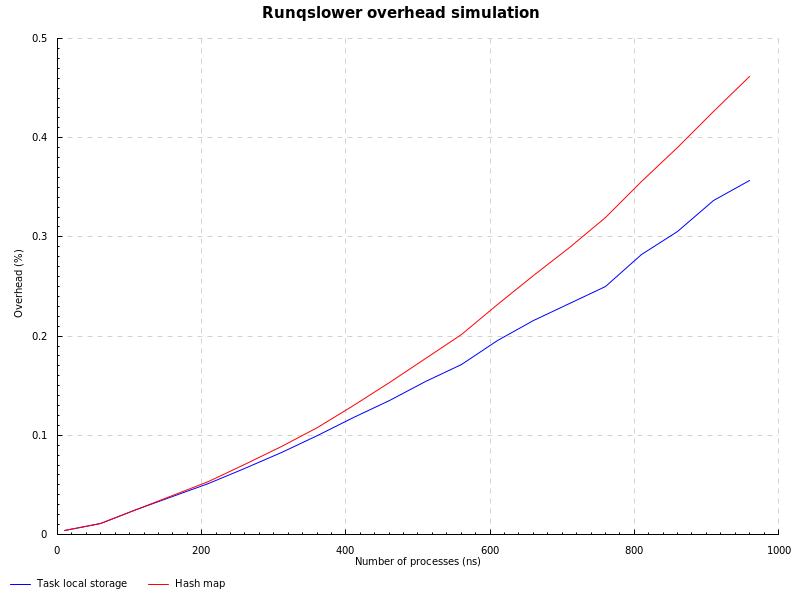
\includegraphics[width=0.65\textwidth,center]{overhead.png}
    \end{center}
\end{frame}
\note{
}

\fontsize{18pt}{18}\selectfont
\begin{frame}
  \vspace*{2.5cm}
  \begin{minipage}[b][\paperheight]{\textwidth}
  \begin{center}

      %\raggedright%
      \linespread{1.0}%
      \usebeamerfont{title}%
      \usebeamercolor[fg]{title}%
      \if@noSmallCapitals%
        Questions?
      \else%
        \scshape{\color{black} Questions?}%
      \fi%
      \vspace*{0.3em}

      \usebeamerfont{subtitle}%
      \fontsize{13pt}{14}\selectfont
      \usebeamercolor[fg]{subtitle}%
        \begin{itemize}[label={}]
            \item {\color{black} \twitter\ @erthalion}
            \item {\color{black} \email\ dmitrii.dolgov at redhat dot com}
        \end{itemize}
      \vspace*{2.5em}%

    \vfill
    \vspace*{2em}
  \end{center}
  \end{minipage}
\end{frame}

\end{document}
